\documentclass{article}
% translate with >> pdflatex -shell-escape <file>

% This file is used as unit test for pgfplots, copyright by Christian Feuersaenger.
% 
% See
%   http://pgfplots.sourceforge.net/pgfplots.pdf
% for pgfplots.
%
% Any required input files (for <plot table> or <plot file> or the table package) can be downloaded
% at
% http://www.ctan.org/tex-archive/graphics/pgf/contrib/pgfplots/doc/latex/
% and
% http://www.ctan.org/tex-archive/graphics/pgf/contrib/pgfplots/doc/latex/plotdata/

\usepackage{pgfplots}
\pgfplotsset{compat=newest}

\pagestyle{empty}

\begin{document}

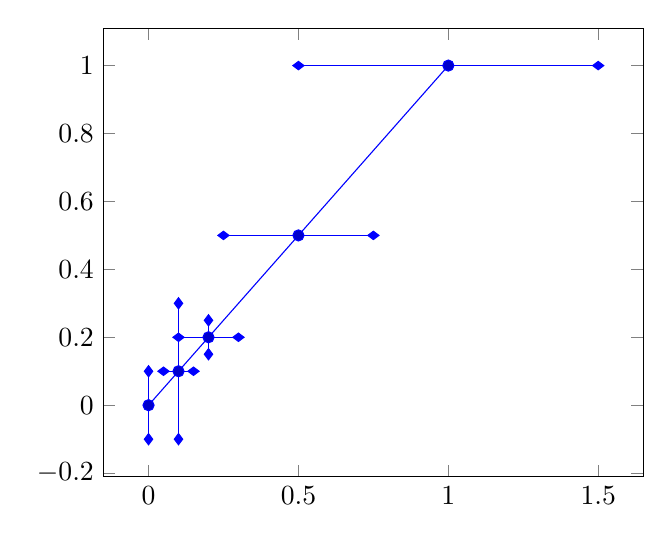
\begin{tikzpicture}
\begin{axis}
\addplot plot[
	error bars/.cd,
	y dir=both,y explicit,
	x dir=both,x fixed relative=0.5,
	error mark=diamond*,
]
	coordinates
	{(0,0) +- (0.5,0.1) 
	(0.1,0.1)  +- (0.05,0.2)
	(0.2,0.2) 	+- (0,0.05)
	(0.5,0.5)
	(1,1)};
\end{axis}
\end{tikzpicture}
\end{document}
